% !TEX encoding = UTF-8 Unicode
\chapter{Descripción del Trabajo Concursos de Programación}

\label{cap:descripcionTrabajoConcursosProgramacion}

\chapterquote{La gente de El Ejido no espera a que las cosas caigan del cielo; allí se arremangan y las sacan ellos mismos de la tierra}{Pepe Navarro.}

El capítulo anterior deja construidas dos piezas fundamentales: un motor capaz de renderizar contenido 3D dentro de OBS y una capa de anclaje AR que permite colocar ese contenido sobre marcadores físicos detectados en tiempo real. Este capítulo parte de esa base y la amplía hacia contenido informativo dinámico para concursos de programación.

Ya hemos descrito cómo integrar realidad aumentada en OBS Studio: imprimir marcadores ArUco sobre cualquier superficie, calibrar la cámara y configurar el filtro para que ancle un modelo 3D al marcador detectado. Ese sistema es completo y funcional por sí solo para cualquier retransmisión que necesite superponer geometría fija sobre la imagen de una
cámara. Sin embargo, aplicarlo a un concurso de programación plantea un requisito distinto: el contenido que debe aparecer sobre el vídeo no es estático sino que cambia continuamente a lo largo de la competición. La clasificación se actualiza con cada envío aceptado, el tiempo restante avanza segundo a segundo y la información del equipo que la cámara está enfocando varía en función de qué mesa está en plano. Un modelo 3D fijo no es suficiente.
 
Como se describió en el capítulo~\ref{cap:concursos_programacion}, un concurso de programación genera un
flujo continuo de información estructurada: los envíos de los equipos modifican la clasificación
en tiempo real, el servidor de jurado mantiene un cronómetro oficial con estados bien definidos
(\textit{running}, \textit{paused}, \textit{frozen}) y cada equipo dispone de metadatos como
nombre, universidad e identificador, que permiten contextualizar cualquier plano de cámara. Toda
esa riqueza informativa queda invisible en una retransmisión convencional a menos que el sistema
de vídeo sea capaz de consumirla y proyectarla directamente sobre la imagen.
 
Este capítulo describe las dos extensiones que convierten el plugin en una herramienta específica
para la retransmisión de concursos. La primera es la incorporación de \textbf{elementos visuales
dinámicos}: un reloj analógico 3D cuyos elementos se mueven fotograma a fotograma y un sistema
de renderizado de texto arbitrario que permite mostrar cualquier información sobre la imagen
anclada a un marcador. Ambos se diseñaron como componentes reutilizables, independientes de
cualquier fuente de datos externa, de modo que funcionan de forma autónoma antes de conectar con
ningún servidor. La segunda extensión es la \textbf{conectividad con DOMjudge}
\citep{DOMjudge}: un cliente HTTP asíncrono que consulta periódicamente la API REST del sistema
de jurado, obtiene la clasificación y el estado de la competición, y alimenta con esos datos los
elementos dinámicos descritos anteriormente.
 
El capítulo se organiza en cinco partes. La sección~\ref{sec:texto_dinamico} describe el sistema
de renderizado de texto dinámico anclado a marcadores. La sección~\ref{sec:reloj3d} presenta el
reloj analógico 3D y su lógica de animación. La sección~\ref{sec:domjudge_integracion} introduce
la conectividad con DOMjudge, la arquitectura asíncrona y los modos de visualización que
alimenta. La sección~\ref{sec:configuracion_ampliada} describe la configuración del servidor y
el mapeo de marcadores. La sección~\ref{sec:conclusiones_diseno_concursos} recoge las conclusiones y
las decisiones de diseño que condicionaron el desarrollo.
 
 
%%=============================================================
\section{Renderizado de texto dinámico}
\label{sec:texto_dinamico}
%%=============================================================
 
Superponer texto sobre un vídeo en tiempo real es técnicamente más exigente que superponer un
modelo 3D estático. Un modelo se carga una vez y se redibuja cada fotograma con la misma geometría,
el texto, en cambio, puede cambiar de contenido en cualquier momento y su tamaño en pantalla
varía según el volumen de información que deba mostrar. A eso se suma el requisito de que el
bloque de texto parezca físicamente anclado al marcador: debe seguir su posición y orientación
con precisión, sin temblores perceptibles, con un fondo legible y con la perspectiva correcta.
 
 
\subsection{Cadena de procesamiento de renderizado}
\label{subsec:pipeline_overlay}
 
La cadena de procesamiento reutiliza la detección descrita en el capítulo anterior: cada fotograma se convierte al
espacio de color de OpenCV, el detector ArUco localiza el marcador elegido y el algoritmo de
Perspectiva-$n$-Puntos calcula su posición y orientación tridimensionales. Las coordenadas de
las esquinas se escalan a la resolución de salida de OBS de forma proporcional:
\[
  s_x = \frac{W_{\text{base}}}{W_{\text{frame}}}, \qquad s_y = \frac{H_{\text{base}}}{H_{\text{frame}}}
\]
garantizando coherencia entre el espacio del detector y el espacio de dibujo de la superposición
con independencia de la resolución real de la cámara.

Lo que este módulo añade sobre el capítulo anterior son tres adaptaciones específicas para el
renderizado de texto. Primera: la proyección ortográfica de OBS se configura con el mismo
convenio de ejes que OpenCV (origen en la esquina superior izquierda, eje $Y$ hacia abajo),
de modo que las coordenadas 2D del detector se usan directamente para posicionar la superposición sin
transformación adicional; la figura~\ref{fig:coordsystems} ilustra la diferencia con el
convenio OpenGL clásico. Segunda: la orientación en representación de Rodrigues que devuelve el
algoritmo PnP se traduce a la pose de la superposición mediante la cadena de transformaciones:
\[
  M = T_{\text{pos}} \cdot R_{\text{offsets}} \cdot R_{\text{flip}} \cdot R_{\text{ArUco}}
  \cdot R_{\text{elev}} \cdot T_{\text{centrado}}
\]
donde $R_{\text{flip}} = R_x(180^\circ)$ corrige la diferencia de convenios de rotación entre
OpenCV y OBS, $R_{\text{ArUco}}$ aplica la orientación real del marcador, $R_{\text{elev}} =
R_x(90^\circ)$ hace que el panel quede erguido sobre él, y $T_{\text{centrado}}$ lo centra
horizontalmente sobre el punto de anclaje. La figura~\ref{fig:rodrigues_pipeline} resume el
proceso de conversión. Cuando la inclinación del marcador se aproxima a la vertical, el sistema
detecta la singularidad de \textit{gimbal lock} y aplica un caso especial: fija la inclinación
al valor límite y deduce el giro restante a partir de los elementos de la matriz de rotación que
aún son fiables, produciendo una orientación estable aunque con pérdida de un grado de libertad.
Tercera: se añade corrección angular para que el texto resulte siempre legible aunque el
marcador esté girado en el plano de la mesa.
 
\begin{figure}[h]
\centering
\begin{tikzpicture}[font=\small, scale=0.95]
  \draw[thick, gray!35] (0,0) rectangle (2.8,-2.2);
  \draw[-{Stealth[length=7pt]}, ultra thick, red!70!black] (0,0) -- (1.8,0) node[right] {$X$};
  \draw[-{Stealth[length=7pt]}, ultra thick, blue!70!black] (0,0) -- (0,-1.8) node[left] {$Y$};
  \fill (0,0) circle (3pt);
  \node[above right, font=\scriptsize] at (0,0) {$(0,0)$};
  \node[below, font=\small\bfseries] at (1.4,-2.5) {OpenCV / OBS configurado};
  \node[below, font=\scriptsize] at (1.4,-3.0) {Origen: esquina superior izquierda};
  \node at (3.7,-1.1) {\Large$\neq$};
  \draw[thick, gray!35] (4.6,-2.2) rectangle (7.4,0);
  \draw[-{Stealth[length=7pt]}, ultra thick, red!70!black] (4.6,-2.2) -- (6.4,-2.2) node[right] {$X$};
  \draw[-{Stealth[length=7pt]}, ultra thick, blue!70!black] (4.6,-2.2) -- (4.6,-0.4) node[left] {$Y$};
  \fill (4.6,-2.2) circle (3pt);
  \node[below right, font=\scriptsize] at (4.6,-2.2) {$(0,0)$};
  \node[below, font=\small\bfseries] at (6.0,-2.5) {OpenGL clásico};
  \node[below, font=\scriptsize] at (6.0,-3.0) {Origen: esquina inferior izquierda};
\end{tikzpicture}
\caption{Convenios de coordenadas 2D. OBS se configura para usar el convenio de OpenCV, de
forma que las coordenadas del detector se pueden usar sin transformación adicional.}
\label{fig:coordsystems}
\end{figure}
 
\begin{figure}[h]
\centering
\resizebox{\linewidth}{!}{%
\begin{tikzpicture}[
    node distance=0.8cm and 2.2cm,
    box/.style={rectangle, rounded corners=4pt, draw=black!60, fill=gray!10,
                minimum width=2.4cm, minimum height=0.9cm, align=center, font=\small},
    arr/.style={-{Stealth[length=7pt]}, thick}
  ]
  \node[box] (rvec)  {\textbf{rvec}\\\scriptsize vector Rodrigues\\$(r_x, r_y, r_z)$};
  \node[box, right=of rvec] (R)    {\textbf{Matriz R}\\\scriptsize rotación $3\times3$};
  \node[box, right=of R]    (euler){\textbf{Euler}\\\scriptsize pitch, yaw, roll};
  \node[box, right=of euler] (pose) {\textbf{Pose}\\\scriptsize orientación\\de la superposición};
  \draw[arr] (rvec)  -- node[midway, above, font=\scriptsize, yshift=3pt] {Rodrigues()} (R);
  \draw[arr] (R)     -- node[midway, above, font=\scriptsize, yshift=3pt] {extracción} (euler);
  \draw[arr] (euler) -- node[midway, above, font=\scriptsize, yshift=3pt] {aplicación} (pose);
\end{tikzpicture}}
\caption{cadena de procesamiento de conversión de la representación de Rodrigues a la orientación de la superposición.}
\label{fig:rodrigues_pipeline}
\end{figure}
 
 
\subsection{Suavizado de la superposición}
\label{subsec:suavizado}
 
Aunque la detección ArUco es robusta, el ruido de la imagen de cámara (granulado del sensor,
compresión de vídeo y microvibraciones) provoca que la posición y el ángulo calculados del
marcador oscilen ligeramente de fotograma a fotograma. Sin ninguna corrección, el texto parece temblar
sobre el vídeo, lo que resulta poco profesional en una retransmisión.
 
Para mitigarlo, el sistema aplica un filtro de suavizado exponencial sobre la posición y el
ángulo de la superposición. En lugar de saltar directamente al valor nuevo detectado en cada fotograma, se
mezcla ese valor con el del fotograma anterior según un factor configurable $\alpha \in (0,\,1]$:
\[
  P_t = (1 - \alpha)\,P_{t-1} + \alpha\,P_{\text{detectado}}
\]
Con $\alpha$ cercano a $1$ la superposición sigue el marcador con mucha fidelidad pero puede mostrar
algo de temblor residual. Con $\alpha$ más pequeño el movimiento es más suave pero tiene algo
más de inercia, por lo que en cámara rápida puede quedarse ligeramente retrasado. El operador
ajusta este parámetro según las condiciones de grabación.
 
El ángulo requiere un tratamiento especial. Si el marcador pasa de estar a $179^\circ$ a
$-179^\circ$, una interpolación directa haría girar la superposición $358^\circ$ en sentido contrario
en lugar de $2^\circ$. El sistema detecta este caso y siempre interpola por el camino angular
más corto entre los dos valores. El suavizado se reinicia automáticamente cuando el marcador
detectado cambia de ID, para no arrastrar la posición del marcador anterior a la animación del
nuevo.


%%=============================================================
\section{El reloj analógico 3D}
\label{sec:reloj3d}
%%=============================================================
 
El segundo elemento dinámico es un reloj analógico de cuenta atrás renderizado como modelo 3D
anclado al marcador. A diferencia del texto, cuyo contenido proviene de una fuente de datos
externa, el reloj es un sistema autónomo: mantiene su propio estado de cuenta atrás y actualiza
la posición angular de sus manecillas fotograma a fotograma a partir del tiempo transcurrido,
sin depender de ninguna conexión exterior para funcionar. Cuando se integra con DOMjudge, puede
sincronizarse con el tiempo oficial del concurso, corrigiendo cualquier deriva acumulada.
 
La lógica del cronómetro reside en el módulo \texttt{countdown\_clock}, que mantiene el estado
de la cuenta atrás (\texttt{STOPPED}, \texttt{RUNNING}, \texttt{PAUSED} o \texttt{FINISHED}),
la duración total configurada en horas, minutos y segundos, y el tiempo restante que se
decrementa fotograma a fotograma. En cada iteración del \textit{callback} de vídeo, el sistema llama a
\texttt{countdown\_clock\_tick} con el tiempo transcurrido desde el fotograma anterior, lo que
actualiza el tiempo restante con alta precisión independientemente de la cadencia de fotogramas.
 
El tiempo restante se traduce en ángulos de rotación para las mallas 3D de las manecillas. El
plugin ofrece dos modos de presentación:
 
\begin{itemize}
    \item \textbf{Tres manecillas:} Cada malla del modelo (hora, minuto y segundo) recibe su
    propio ángulo calculado de forma análoga a un reloj analógico clásico. La manecilla de
    segundos avanza $6^\circ$ por segundo, la de minutos $6^\circ$ por minuto completado y la
    de horas divide proporcionalmente el rango configurado del cuadrante.
    \item \textbf{Manecilla única:} Una sola malla barre $360^\circ$ a lo largo de la duración
    total configurada, de modo que su posición angular representa qué fracción del tiempo total
    ha transcurrido, como un indicador de progreso circular.
\end{itemize}
 
La posición del reloj puede fijarse manualmente en pantalla o anclarse a un marcador ArUco,
seleccionando el modo \textbf{Countdown} en el panel de propiedades.
 
 
%%=============================================================
\section{Conectividad con DOMjudge}
\label{sec:domjudge_integracion}
%%=============================================================
 
Los elementos dinámicos descritos en las secciones anteriores son componentes de renderizado que
operan sobre datos. En una retransmisión de concurso esos datos deben proceder del sistema de
jurado en tiempo real. Esta sección describe cómo el plugin obtiene esa información, cómo la
distribuye a cada componente y qué modos de visualización ofrece al operador.
 
 
\subsection{Arquitectura de hilos}
\label{subsec:hilos}
 
El plugin separa las responsabilidades en dos contextos de ejecución para garantizar que ninguna
operación costosa bloquee la salida de vídeo.
 
El \textbf{hilo principal} es gestionado íntegramente por OBS Studio. Sobre él recaen los tres
tipos de \textit{callbacks} que el plugin registra: el \textit{callback} de vídeo, que ejecuta la
detección ArUco en cada fotograma entrante; el \textit{callback} de renderizado, que construye la salida
visual; y las actualizaciones de la interfaz de usuario. Dado que los tres comparten el mismo
hilo, la implementación evita cualquier operación bloqueante dentro de ellos.
 
El \textbf{hilo secundario} lo crea el propio plugin al activarse la conectividad web mediante
\texttt{pthread\_create}. Este hilo ejecuta un bucle que lanza peticiones HTTP a DOMjudge a
intervalos configurables, duerme entre consultas y escribe los resultados en una estructura
compartida protegida por un \texttt{pthread\_mutex\_t}. El acceso a esa caché se sincroniza con
\texttt{pthread\_mutex\_lock} y \texttt{pthread\_mutex\_unlock}, de modo que el hilo principal
únicamente lee el último resultado disponible sin bloquear el renderizado durante las operaciones
de red.
\begin{figure}[H]
\centering
\begin{tikzpicture}[
    font=\small,
    node distance=1.4cm,
    arr/.style={-{Stealth[length=7pt]}, thick},
    box/.style={draw, rounded corners, minimum width=5.5cm, minimum height=1cm, align=center},
    cache/.style={draw, rounded corners, fill=yellow!15, minimum width=4.2cm,
                  minimum height=0.85cm, align=center, font=\scriptsize}
  ]
  \node[box, fill=blue!8]
    (main) {\textbf{Hilo principal (OBS)}\\{\scriptsize vídeo · renderizado · UI}};
  \node[cache, below=1.3cm of main]
    (cache) {\textbf{Caché compartida}\\{\tiny\texttt{pthread\_mutex\_t}}};
  \node[box, fill=orange!10, below=1.3cm of cache]
    (sec) {\textbf{Hilo secundario (plugin)}\\{\scriptsize peticiones HTTP · libcurl}};
  %% hilo secundario escribe → caché
  \draw[arr] (sec.north west) to[bend left=20]
    node[left, font=\scriptsize] {escribe} (cache.south west);
  %% caché → hilo principal lee
  \draw[arr] (cache.north west) to[bend left=20]
    node[left, font=\scriptsize] {lee} (main.south west);
  %% hilo principal señal de parada → hilo secundario
  \draw[arr] (main.south east) to[bend right=20]
    node[right, font=\scriptsize, align=left] {señal de\\parada} (sec.north east);
\end{tikzpicture}
\caption{Arquitectura de dos hilos del plugin. El hilo secundario realiza peticiones HTTP
asíncronas y escribe los datos en la caché protegida por un \texttt{pthread\_mutex\_t}, el
hilo principal de OBS lee de la caché en cada fotograma sin bloquearse.}
\label{fig:hilos}
\end{figure}
 
Cuando el plugin se destruye, se señaliza al hilo secundario para que termine de forma limpia
antes de liberar los recursos. Las contraseñas de la API se sobrescriben en memoria antes de
ser liberadas, evitando que queden trazas en el \textit{heap} del proceso. Esta secuencia amplía
el ciclo de vida descrito en la sección~\ref{sec:ciclo_vida}: la inicialización ahora también
crea el hilo secundario cuando la conectividad está habilitada, y la destrucción añade una señal
de parada que garantiza que el hilo secundario termine antes de liberar cualquier recurso
compartido.
 
 
\subsection{Red asíncrona con libcurl}
\label{subsec:libcurl}
 
El módulo de red se basa en la biblioteca \textbf{libcurl} y opera íntegramente en el hilo
secundario. El hilo principal de OBS nunca espera la respuesta del servidor; simplemente lee el
último resultado disponible en la caché compartida cuando lo necesita.
 
El sistema implementa políticas de \textit{timeout} y reintentos con espera exponencial. Si el
servidor DOMjudge cae, el plugin sigue funcionando con los últimos datos guardados en caché, sin
mostrar información vacía ni congelar la emisión.
 
 
\subsection{Máquina de estados de conexión}
\label{subsec:estados_conexion}
 
La comunicación con el servidor se gestiona mediante una \textbf{máquina de estados} que
garantiza la estabilidad del plugin incluso si la red falla. El sistema transita entre
\texttt{DISCONNECTED}, \texttt{CONNECTING}, \texttt{CONNECTED} y \texttt{FAILED}, y el estado
actual se muestra en el panel de OBS para que el operador sepa en todo momento si los datos son
frescos o proceden de la caché. Si la conexión falla, el plugin espera intervalos crecientes
antes de intentar reconectar (\textit{backoff} exponencial), reduciendo la carga sobre el
servidor en situaciones de sobrecarga.
 
 
\subsection{Endpoints y flujo de datos}
\label{subsec:endpoints}
 
El plugin consulta periódicamente tres puntos clave de la API REST de DOMjudge:
 
\begin{enumerate}
    \item \textbf{/contests:} Metadatos del torneo y tiempo transcurrido y restante, para
    sincronizar el cronómetro 3D con la cuenta atrás oficial.
    \item \textbf{/teams:} Lista de participantes con sus nombres reales y afiliaciones
    universitarias.
    \item \textbf{/scoreboard:} Ranking actual, problemas resueltos y tiempo de penalización de
    cada equipo.
\end{enumerate}
 
El módulo \texttt{json\_utils} deserializa estas respuestas y las convierte en estructuras de C
listas para ser consumidas por el motor de renderizado. El intervalo de consulta es configurable;
un valor de 30 segundos es suficiente para mantener el scoreboard actualizado en la mayoría de
concursos. Una vez desserializados, los datos fluyen hacia los dos componentes dinámicos: el
tiempo oficial va al reloj analógico, que corrige su deriva interna y ajusta su estado (activo,
pausado o detenido); los datos de equipos y clasificación van al motor de texto, que los
presenta en los modos Scoreboard y Team Info. La figura~\ref{fig:flujo_datos} resume este flujo.
 
\begin{figure}[H]
\centering
\resizebox{\linewidth}{!}{%
\begin{tikzpicture}[font=\small,
    arr/.style={-{Stealth[length=7pt]}, thick},
    box/.style={draw, rounded corners, minimum height=0.85cm, align=center},
    node distance=0.5cm and 1.6cm]
  \node[box, fill=green!8,   minimum width=2.8cm] (dj)
    {\textbf{DOMjudge}\\{\scriptsize API REST}};
  \node[box, fill=orange!10, minimum width=2.8cm, right=1.8cm of dj] (curl)
    {\textbf{Hilo secundario}\\{\scriptsize libcurl}};
  \node[box, fill=gray!12,   minimum width=2.8cm, right=1.8cm of curl] (cache)
  {\textbf{Caché}\\{\scriptsize pthread\_mutex\_t}};
  \node[box, fill=blue!8,    minimum width=2.8cm, above right=0.5cm and 1.6cm of cache] (clock)
    {\textbf{Reloj 3D}\\{\scriptsize Countdown}};
  \node[box, fill=blue!8,    minimum width=2.8cm, below right=0.5cm and 1.6cm of cache] (score)
    {\textbf{Motor de texto}\\{\scriptsize Scoreboard · Team Info}};
  \draw[arr] (dj)    -- node[above, font=\scriptsize] {HTTP} (curl);
  \draw[arr] (curl)  -- node[above, font=\scriptsize] {escritura} (cache);
  \draw[arr] (cache) -- node[above, font=\scriptsize, sloped] {lectura} (clock);
  \draw[arr] (cache) -- node[below, font=\scriptsize, sloped] {lectura} (score);
\end{tikzpicture}%
}
\caption{Flujo de datos desde DOMjudge hasta los componentes de renderizado. El hilo secundario
escribe en la caché; el hilo principal la lee sin bloqueos para alimentar el reloj y el motor
de texto.}
\label{fig:flujo_datos}
\end{figure}
 
 
\subsection{Modos de visualización}
\label{subsec:modos}
 
Con los datos en caché, el plugin ofrece cuatro modos de operación seleccionables desde el panel
de propiedades:
 
\begin{itemize}
    \item \textbf{Modelo 3D:} Modo estándar de RA descrito en el capítulo anterior. No requiere
    conectividad con DOMjudge.

    \begin{figure}[H]
      \centering
      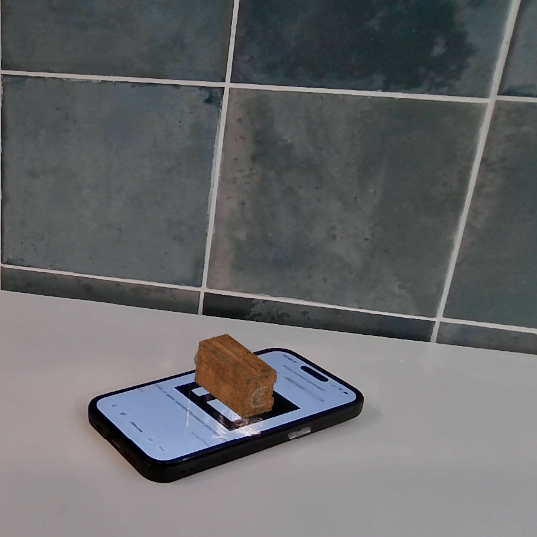
\includegraphics[width=0.82\textwidth]{Imagenes/Vectorial/ModoAr}
      \caption{Modo modelo 3D: geometría virtual anclada y orientada sobre el marcador ArUco en tiempo real.}
      \label{fig:modo_ar_concursos}
    \end{figure}

    \item \textbf{Cronómetro:} Reloj analógico 3D de cuenta atrás sincronizado con el tiempo oficial
    del concurso. Puede anclarse a un marcador ArUco o posicionarse manualmente en pantalla.

    \item \textbf{Marcador de clasificación:} Tabla de clasificación general organizada en cuatro columnas
    (posición, nombre del equipo, problemas resueltos y tiempo de penalización). Cada columna es
    una fuente de texto independiente cuyos anchos se adaptan automáticamente al contenido, sin
    riesgo de desbordamiento. Puede mostrarse en pantalla completa o anclado a un marcador.

    \begin{figure}[H]
      \centering
      \includegraphics[width=0.82\textwidth]{Imagenes/Vectorial/usoScoreboard}
      \caption{Modo marcador de clasificación: tabla de equipos proyectada sobre el vídeo en tiempo real durante el concurso.}
      \label{fig:modo_scoreboard}
    \end{figure}

    \item \textbf{Información de equipo:} Muestra la información del equipo cuyo marcador está visible en
    cámara en ese instante. Si no hay ningún marcador registrado en plano, la superposición desaparece
    hasta que la cámara vuelva a enfocar una mesa registrada.

\begin{figure}[H]
  \centering
  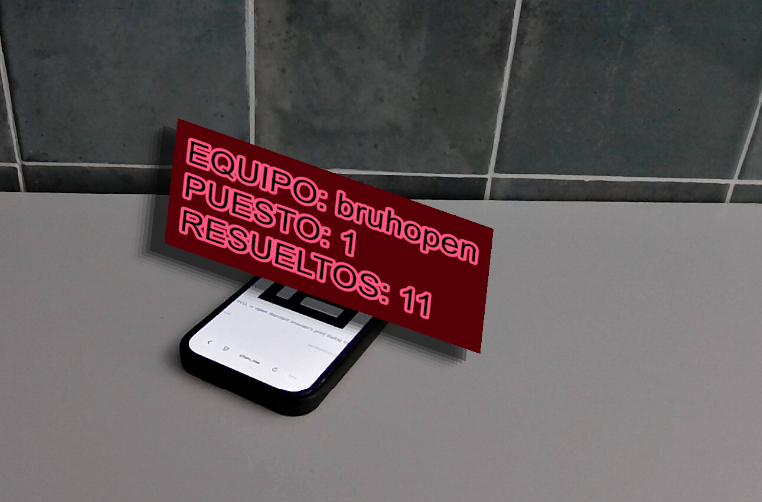
\includegraphics[width=0.82\textwidth]{Imagenes/Vectorial/ModoTeamInfo}
      \caption{Modo información de equipo: datos del equipo detectado superpuestos sobre el vídeo en tiempo real.}
      \label{fig:modo_teaminfo}
\end{figure}

\end{itemize}

El panel también expone controles de visibilidad que permiten activar o desactivar capas de
información de forma independiente sin interrumpir la emisión.
 
 
%%=============================================================
\section{Configuración ampliada}
\label{sec:configuracion_ampliada}
%%=============================================================
 
La conectividad con DOMjudge requiere ampliar la interfaz con dos grupos de parámetros nuevos:
el acceso al servidor y el mapeo entre los marcadores físicos y los equipos del concurso.
 
 
\subsection{Configuración del servidor}
\label{subsec:config_servidor}
 
El acceso a los datos de la competición requiere tres parámetros en el panel de propiedades. La
\textbf{URL base} permite cambiar entre el servidor de producción del concurso y un entorno de
prueba sin modificar el código fuente. El \textbf{identificador del torneo} filtra los datos del
servidor para obtener únicamente la información del evento actual mediante su ID en DOMjudge.
La \textbf{autenticación} se implementa mediante \textit{HTTP Basic Auth}; las credenciales se
almacenan a través de la API de persistencia de OBS Studio, evitando que queden en texto plano
en el archivo de configuración de la escena.

\begin{figure}[H]
  \centering
  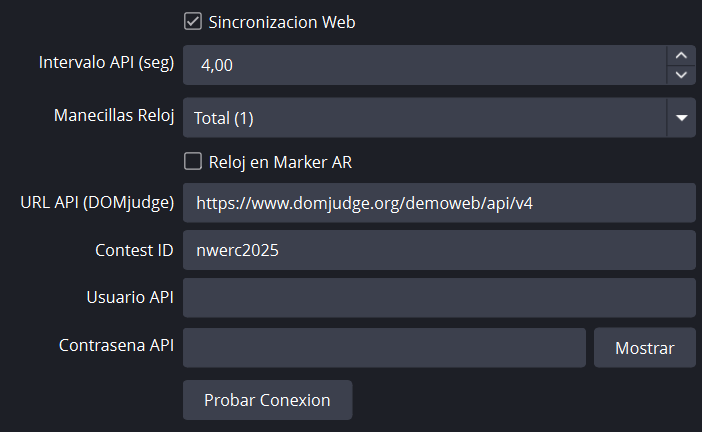
\includegraphics[width=0.72\textwidth]{Imagenes/Vectorial/UI_ConexionWeb}
  \caption{Panel de configuración de la conexión con DOMjudge: URL base, identificador del torneo y credenciales de autenticación.}
  \label{fig:ui_conexion_web}
\end{figure}


\subsection{Mapeo de marcadores a equipos}
\label{subsec:mapeo}
 
La funcionalidad que vincula el mundo físico con los datos digitales es el \textbf{fichero de
mapeo}: un archivo JSON que el operador prepara antes de la retransmisión y que asocia cada ID
de marcador ArUco impreso en las mesas del concurso con el identificador del equipo
correspondiente en DOMjudge:
 
\begin{verbatim}
[
  { "marker_id": 1, "team_id": "42" },
  { "marker_id": 2, "team_id": "12" },
  { "marker_id": 5, "team_id": "7"  }
]
\end{verbatim}
 
Al cargar el fichero, el módulo de sincronización construye en memoria la tabla de mapeos y
extrae la lista de IDs de marcador válidos, que el módulo de detección usa para filtrar los
marcadores detectados en cada fotograma y descartar los que no corresponden a ningún equipo
registrado. El fichero puede recargarse sin reiniciar la escena. Cuando hay varios marcadores
simultáneos en pantalla, el modo Team Info elige el primero en el orden en que el detector los
devuelve; si se necesitara mostrar varios equipos a la vez, basta con añadir una instancia del
filtro por equipo, trabajando en paralelo sin interferencias.
 
 
%%=============================================================
\section{Conclusiones y decisiones de diseño}
\label{sec:conclusiones_diseno_concursos}
%%=============================================================
 
El trabajo descrito en este capítulo extiende el plugin de realidad aumentada con tres
capacidades nuevas: renderizado de texto dinámico anclado a marcadores, un reloj analógico 3D
sincronizado y conectividad con la API de DOMjudge. La combinación de los tres convierte una
herramienta de superposición genérica en un sistema orientado específicamente a la retransmisión
de concursos de programación.
 
A lo largo del desarrollo se tomaron tres decisiones que condicionan directamente la estabilidad
del sistema durante una retransmisión real. La primera fue usar consultas periódicas con libcurl
en lugar de mecanismos de suscripción más complejos. Esta opción reduce el riesgo operativo y
simplifica el diagnóstico cuando hay incidencias de red, a costa de una latencia de actualización
acotada por el intervalo de consulta, que en la práctica resulta imperceptible para el espectador.
 
La segunda decisión fue mantener un modo degradado con caché local. Si la conexión falla, el
plugin no deja de renderizar ni muestra paneles vacíos: continúa con el último estado conocido
y vuelve a sincronizar en cuanto el servidor responde de nuevo. Para una realización en directo,
esta continuidad visual es más valiosa que forzar una reconexión agresiva que podría interrumpir
la imagen durante varios fotogramas.
 
La tercera fue centralizar toda la configuración en el panel de OBS. La URL del servidor, el
identificador del concurso, las credenciales de acceso, el intervalo de consulta y el mapeo
JSON de marcadores a equipos se ajustan en caliente desde la interfaz, sin necesidad de
reiniciar la escena ni detener la emisión. Esto permite al operador corregir cualquier parámetro
durante el propio evento, lo que resulta especialmente útil cuando la infraestructura de red
cambia entre la fase de preparación y el inicio de la retransmisión.
 
\begin{sloppypar}
La implementación del hilo secundario usa la interfaz \textit{POSIX threads}
(\texttt{pthread\_create}, \texttt{pthread\_mutex\_init}, \texttt{pthread\_mutex\_lock},
\texttt{pthread\_mutex\_unlock} y \texttt{pthread\_join}) para separar las peticiones HTTP del
hilo principal de OBS. En la implementación actual, toda la sincronización de la caché
compartida se concentra en un mutex único alrededor de los datos de concurso y scoreboard. En
Windows esta interfaz se resuelve mediante la dependencia \texttt{w32-pthreads} que arrastra
\textit{libobs}, de manera que el código mantiene una API de concurrencia homogénea en C sin
usar primitivas Win32 directas.
\end{sloppypar}
